% !TEX root = ../chatbot-report.tex
%
\chapter{Dữ liệu}
\label{sec:data}

\section{Dữ liệu}
Dữ liệu được dùng là \textit{\detokenize{Cornell Movie-Dialogs Corpus <https://www.cs.cornell
.edu/~cristian/Cornell_Movie-Dialogs_Corpus.html>}} là một bộ dữ liệu đa dạng chứa các đoạn hội thoại của nhân vật:
\begin{itemize}
    \item 220.579 hội thoại giữa 10.292 cặp nhân vật trong phim.
    \item 9.035 nhân vật từ 617 phim.
    \item 304,713 câu thoại
\end{itemize}
Bộ dữ liệu này rất lớn và đa dạng, và có sự khác biệt lớn về hình thức ngôn ngữ, khoảng thời gian, cảm xúc.

\textbf{File: movie\detokenize{_}lines.txt} \\
File này thông tin các câu hội thoại của từng nhân vật. Một số dòng dữ liệu mẫu
\begin{displayquote}
b'L1045 \detokenize{+++$+++} u0 \detokenize{+++$+++} m0 \detokenize{+++$+++} BIANCA \detokenize{+++$+++} They do not!\n' \\
b'L1044 \detokenize{+++$+++}  u2 \detokenize{+++$+++}  m0 \detokenize{+++$+++}  CAMERON \detokenize{+++$+++}  They do to!\n' \\
b'L985 \detokenize{+++$+++}  u0 \detokenize{+++$+++}  m0 \detokenize{+++$+++}  BIANCA \detokenize{+++$+++}  I hope so.\n' \\
b'L984 \detokenize{+++$+++}  u2 \detokenize{+++$+++}  m0 \detokenize{+++$+++}  CAMERON \detokenize{+++$+++}  She okay?\n' \\
b"L925 \detokenize{+++$+++}  u0 \detokenize{+++$+++}  m0 \detokenize{+++$+++}  BIANCA \detokenize{+++$+++}  Let's go.\n" \\
b'L924 \detokenize{+++$+++}  u2 \detokenize{+++$+++}  m0 \detokenize{+++$+++}  CAMERON \detokenize{+++$+++}  Wow\n' \\
b"L872 \detokenize{+++$+++}  u0 \detokenize{+++$+++}  m0 \detokenize{+++$+++}  BIANCA \detokenize{+++$+++}  Okay -- you're gonna need to learn how to lie.\n" \\
b'L871 \detokenize{+++$+++}  u2 \detokenize{+++$+++}  m0 \detokenize{+++$+++}  CAMERON \detokenize{+++$+++}  No\n' \\
b'L870 \detokenize{+++$+++}  u0 \detokenize{+++$+++}  m0 \detokenize{+++$+++}  BIANCA \detokenize{+++$+++}  I\'m kidding.  You know how sometimes you just become this
"persona"?  And you don\'t know how to quit?\n' \\
b'L869 \detokenize{+++$+++}  u0 \detokenize{+++$+++}  m0 \detokenize{+++$+++}  BIANCA \detokenize{+++$+++}  Like my fear of wearing pastels?\n' \\
\end{displayquote}
Các trường dữ liệu được phân cách bởi ký hiệu "\detokenize{+++$+++} ".
Các trường lần lượt là:
\begin{itemize}
    \item Mã dòng
    \item Mã nhân vật.
    \item Mã phim
    \item Tên nhân vật
    \item Lời thoại
\end{itemize}

Ví dụ
\begin{displayquote}
L1045 \detokenize{+++$+++} u0 \detokenize{+++$+++} m0 \detokenize{+++$+++} BIANCA \detokenize{+++$+++} They do not!\n' \\
\end{displayquote}
Có nghĩa tại phim có mã 'm0' nhân vật 'u0' có tên là 'BIANCA' nói lời thoại "They do not!"

\textbf{File: movie\detokenize{_}conversations.txt} \\
File này thông tin các câu nào tạo thành một đoạn hội thoại. Một số dòng dữ liệu mẫu
\begin{displayquote}
    u0 \detokenize{+++$+++} u2 \detokenize{+++$+++} m0 \detokenize{+++$+++} ['L870', 'L871', 'L872'] \\
    u0 \detokenize{+++$+++} u2 \detokenize{+++$+++} m0 \detokenize{+++$+++} ['L924', 'L925'] \\
    u0 \detokenize{+++$+++} u2 \detokenize{+++$+++} m0 \detokenize{+++$+++} ['L984', 'L985'] \\
\end{displayquote}
Các trường dữ liệu được phân cách bởi ký hiệu "\detokenize{+++$+++} ".
Các trường lần lượt là:
\begin{itemize}
    \item Mã nhân vật đầu tiên của cuộc hội thoại.
    \item Mã nhân vật thứ hai của cuộc hội thoại.
    \item Mã phim mà cuộc hội thoại diễn ra
    \item Mã lời thoại trong file \textit{movie\detokenize{_}lines.txt}} theo thứ tự để tạo thành cuộc hội thoại
\end{itemize}

Ví dụ
\begin{displayquote}
    u0 \detokenize{+++$+++} u2 \detokenize{+++$+++} m0 \detokenize{+++$+++} ['L870', 'L871', 'L872']
\end{displayquote}
Có nghĩa tại phim có mã 'm0' nhân vật 'u0' và 'u2' nói chuyện với nhau bằng các lời thoại ['L870', 'L871', 'L872']

\section{Tiền xử lý dữ liệu}
\textbf{1. Gộp thông tin} \\
Dựa vào thông tin trên file \textit{movie\detokenize{_}conversations.txt} và \textit{movie\detokenize{_}line.txt}, ta có gộp lại và tạo thành
các câu trong đoạn hội thoại

Ví dụ:
\textit{File: movie\detokenize{_}line.txt}
\begin{displayquote}
b"L872 \detokenize{+++$+++}  u0 \detokenize{+++$+++}  m0 \detokenize{+++$+++}  BIANCA \detokenize{+++$+++}  Okay -- you're gonna need to learn how to lie.\n" \\
b'L871 \detokenize{+++$+++}  u2 \detokenize{+++$+++}  m0 \detokenize{+++$+++}  CAMERON \detokenize{+++$+++}  No\n' \\
b'L870 \detokenize{+++$+++}  u0 \detokenize{+++$+++}  m0 \detokenize{+++$+++}  BIANCA \detokenize{+++$+++}  I\'m kidding.  You know how sometimes you just become this
"persona"?  And you don\'t know how to quit?\n' \\
\end{displayquote}
\textit{File: movie\detokenize{_}conversations.txt}
\begin{displayquote}
    u0 \detokenize{+++$+++} u2 \detokenize{+++$+++} m0 \detokenize{+++$+++} ['L870', 'L871', 'L872']
\end{displayquote}

Sẽ tạo thành đoạn hội thoại sau:
\begin{displayquote}
    (1) Like my fear of wearing pastels? \\
    (2) I'm kidding.  You know how sometimes you just become this "persona"?  And you don't know how to quit? \\
    (3) No \\
\end{displayquote}

\textbf{2. Làm sạch dữ liệu} \\
Đầu tiên chuyển unicode sang ASCII.\\
    \centerline{\textit{I am Heró \(\mapsto\) I am Hero}} \\
Tiếp đó chuyển tất cả các chữ thành chữ thường và loại bỏ các kí tự không phải chữ cái ( ngoại trừ các dấu câu ). \\
    \centerline{\textit{I am Hero  \(\mapsto\) i am hero}} \\
Cuối cùng đễ hỗ trợ training convergence, lọc ra những câu có độ dài vượt ngưỡng 10 \\
%    \centerline{\textit{this sentence is over ten word count bla bla bla bla bla  \(\mapsto\ \emptyset) }} \\

\textbf{3. Xây dựng cặp câu vấn đáp} \\
Với mỗi đoạn hội thoại, lấy 2 câu kế tiếp nhau tạo thành một cặp.\\
Như đoạn hội thoại sau
\begin{displayquote}
    (1) Like my fear of wearing pastels? \\
    (2) I'm kidding.  You know how sometimes you just become this "persona"?  And you don't know how to quit? \\
    (3) No \\
\end{displayquote}
Câu (1)-(2) thành một cặp (2)-(3) thành một cặp.

\textbf{4. Xây dựng từ điển} \\
Việc tiếp theo là tạo ra vocabulary và tải các từ vựng và các cặp câu đôi thoại vào bộ nhớ.

Lưu ý rằng chúng ta đang xử lý các chuỗi từ, không có một ánh xạ ngầm đến một không gian số rời rạc. Như vậy, chúng ta
phải tạo ra một bằng cách ánh xạ từng từ duy nhất mà chúng ta bắt gặp trong tập dữ liệu của mình thành một giá trị chỉ số.
Với một bộ dữ liệu khác nhau thì việc ánh xạ sẽ khác nhau.

Việc sẽ bắt đầu xây dựng từ điển bằng việc với 3 ký tự đặc biệt: \\
PAD\detokenize{_}token \(\mapsto\) 0 \textit{     Dùng cho các câu ngắn} \\
SOS\detokenize{_}token \(\mapsto\) 1 \textit{     Đánh dấu bắt đầu câu} \\
EOS\detokenize{_}token \(\mapsto\) 2 \textit{     Đánh dấu kết thúc câu. Dùng trong thiết lập đầu vào của Decoder} \\

Sau đó với mỗi từ trong cặp hội thoại ta thêm từ đó vào từ điển bằng cách kiểm tra từ điển có từ hay chưa. Nếu có thì
tăng chỉ số đếm từ là 1, còn chưa thì lưu lại từ và ánh xạ tới số tương ứng. \\
\begin{figure}[!htb]
    \center{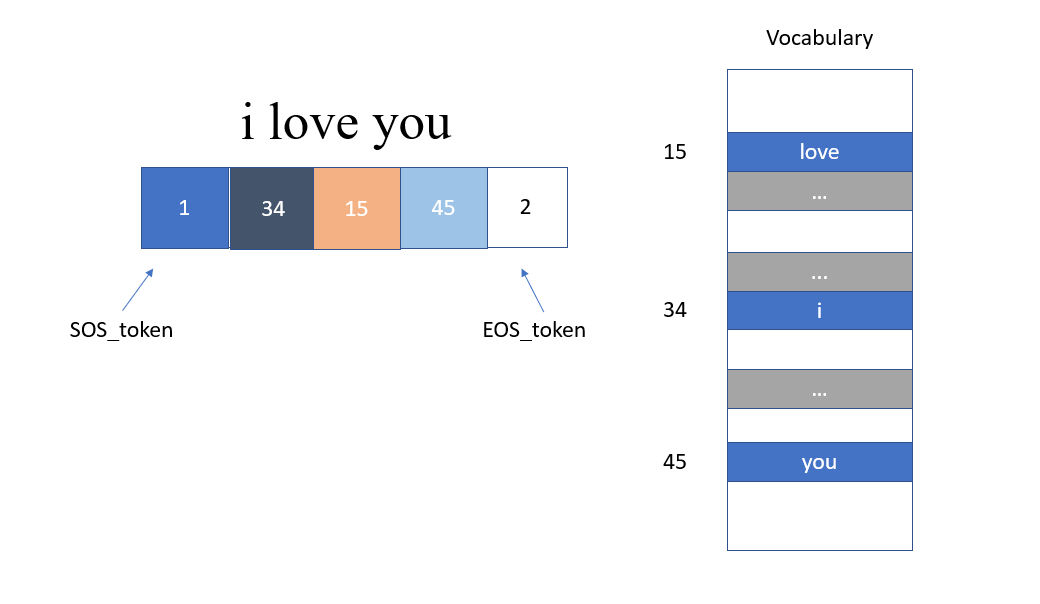
\includegraphics[width=\figureBigSize]
    {figure/data/no_padding.png}}
    \caption{\label{fig:no_padding} Mô tả từ vựng.}
\end{figure}
Trong một số trường hợp câu quá ngắn không phù hợp với model thì chêm PAD\detokenize{_}token cho đủ độ dài. \\
\begin{figure}[!htb]
    \center{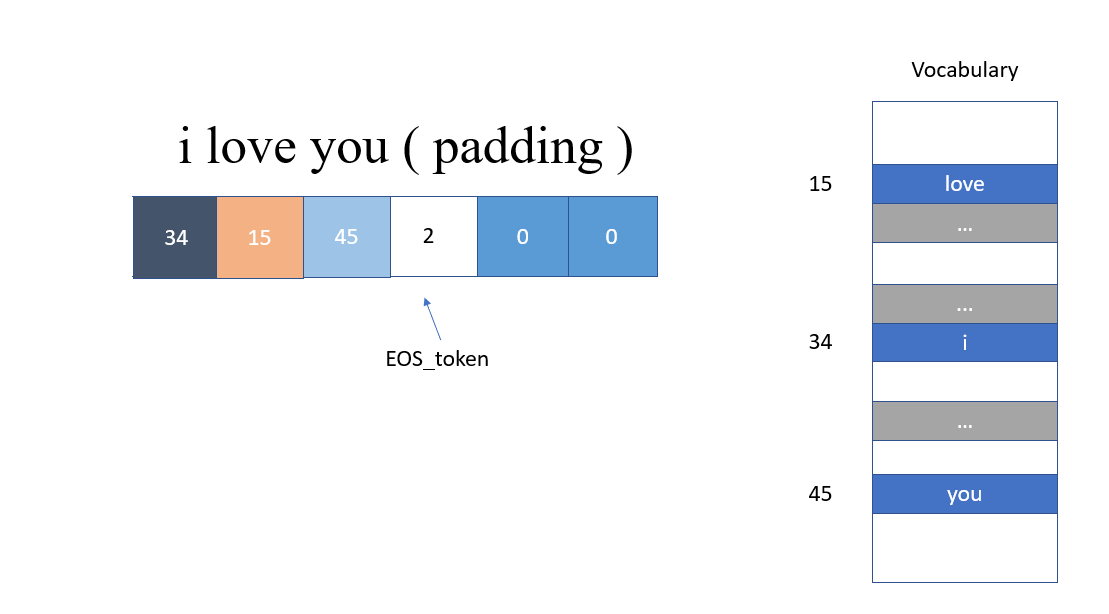
\includegraphics[width=\figureBigSize]
    {figure/data/padding.png}}
    \caption{\label{fig:no_padding} Padding.}
\end{figure}
Một kĩ thuật khác có lợi để đạt được convergence nhanh hơn trong thời gian training là xóa bỏ các từ không được sử dụng nhiều trong vocabulary. Giảm không gian tính năng cũng sẽ làm giảm bớt độ khó của chức năng model phải học cách gần đúng :

1) Xóa bỏ những từ có số lần sử dụng dưới ngưỡng \\
2) Lọc các cặp đối thoại có từ đã được xóa bỏ trong vocabulary \\